\documentclass{beamer}
\usepackage[utf8]{inputenc}

\usetheme{Madrid}
\usecolortheme{default}
\usepackage{amsmath,amssymb,amsfonts,amsthm}
\usepackage{txfonts}
\usepackage{physics}
\usepackage{tkz-euclide}
\usepackage{listings}
\usepackage{adjustbox}
\usepackage{array}
\usepackage{tabularx}
\usepackage{lmodern}
\usepackage{circuitikz}
\usepackage{tikz}
\usepackage{graphicx}

\setbeamertemplate{page number in head/foot}[totalframenumber]

\usepackage{tcolorbox}
\tcbuselibrary{minted,breakable,xparse,skins}

% Background color for code boxes
\definecolor{bg}{gray}{0.95}
\DeclareTCBListing{mintedbox}{O{}m!O{}}{%
  breakable=true,
  listing engine=minted,
  listing only,
  minted language=#2,
  minted style=default,
  minted options={%
    linenos,
    gobble=0,
    breaklines=true,
    fontsize=\small,
    numbersep=8pt,
    #1},
  boxsep=0pt,
  left skip=0pt,
  right skip=0pt,
  left=25pt,
  right=0pt,
  top=3pt,
  bottom=3pt,
  arc=5pt,
  leftrule=0pt,
  rightrule=0pt,
  bottomrule=2pt,
  toprule=2pt,
  colback=bg,
  colframe=orange!70,
  enhanced,
  overlay={%
    \begin{tcbclipinterior}
    \fill[orange!20!white] (frame.south west) rectangle ([xshift=20pt]frame.north west);
    \end{tcbclipinterior}},
}

% Set listings settings for C language
\lstset{
    language=C,
    basicstyle=\ttfamily\small,
    keywordstyle=\color{blue},
    stringstyle=\color{orange},
    commentstyle=\color{green!60!black},
    numbers=left,
    numberstyle=\tiny\color{gray},
    breaklines=true,
    showstringspaces=false,
}

% Define command for column vector and bold vector letter
\newcommand{\myvec}[1]{\ensuremath{\begin{pmatrix}#1\end{pmatrix}}}
\renewcommand{\vec}[1]{\boldsymbol{#1}} % bold vectors

% Meta Info
\title{4.6.5}
\date{September, 2025}
\author{Mahesh Chollangi - EE25BTECH11017}

\begin{document}

\frame{\titlepage}

\section*{Question}
\begin{frame}{Question}
Find the equation of the line passing through point \(\vec{A} = (2,1,-1)\) and parallel to the line. \[\vec{r} = (\vec{i} + \vec{j}) + \lambda(2\vec{i} - \vec{j} + \vec{k}).\]
Also, find the distance between these two lines.
\end{frame}

\begin{frame}{Direction Vector}
The direction vector \(\vec{m}\) of the given line is
\begin{align}
\vec{m} = \myvec{2 \\ -1 \\ 1}
\end{align}

The point through which the required line passes is 
\begin{align}
\vec{A} = \myvec{2 \\ 1 \\ -1}
\end{align}
\end{frame}

\begin{frame}{Equation of the Lines}
The equation of the required line is:
\begin{align}
\vec{r}_1 = \vec{A} + \lambda \vec{m} = \myvec{2 \\ 1 \\ -1} + \lambda \myvec{2 \\ -1 \\ 1}
\end{align}

The equation of the given line is:
\begin{align}
\vec{r}_2 = \myvec{1 \\ 1 \\ 0} + \mu \myvec{2 \\ -1 \\ 1}
\end{align}
\end{frame}

\begin{frame}{Distance Between the Lines}
The distance \(d\) between the two parallel lines with the same direction vector \(\vec{m}\) is:
\begin{align}
d = \frac{\norm{(\vec{A} - \vec{B}) \times \vec{m}}}{\norm{\vec{m}}}
\end{align}
where 
\[
\vec{B} = \myvec{1 \\ 1 \\ 0}.
\]
\end{frame}

\begin{frame}{Compute Vector Difference}
Calculate the vector difference:
\begin{align}
\vec{A} - \vec{B} = \myvec{2 \\ 1 \\ -1} - \myvec{1 \\ 1 \\ 0} = \myvec{1 \\ 0 \\ -1}
\end{align}
\end{frame}

\begin{frame}{Cross Product Calculation}
Calculate the cross product \((\vec{A} - \vec{B}) \times \vec{m}\):
\[
\begin{vmatrix}
\vec{i} & \vec{j} & \vec{k} \\
1 & 0 & -1 \\
2 & -1 & 1
\end{vmatrix}
\]

Expanding:
\begin{align}
&= \vec{i}(0 \times 1 - (-1) \times (-1)) - \vec{j}(1 \times 1 - (-1) \times 2) + \vec{k}(1 \times (-1) - 0 \times 2) \\
&= \vec{i}(0 - 1) - \vec{j}(1 + 2) + \vec{k}(-1 - 0) \\
&= -\vec{i} - 3\vec{j} - \vec{k}
\end{align}
\end{frame}

\begin{frame}{Magnitude Calculations}
Magnitude of the cross product:
\begin{align}
\norm{(\vec{A} - \vec{B}) \times \vec{m}} = \sqrt{(-1)^2 + (-3)^2 + (-1)^2} = \sqrt{11}
\end{align}

Magnitude of the direction vector:
\begin{align}
\norm{\vec{m}} = \sqrt{2^2 + (-1)^2 + 1^2} = \sqrt{6}
\end{align}
\end{frame}

\begin{frame}{Final Distance and Conclusion}
Hence, the distance between the two lines is:
\begin{align}
d = \frac{\sqrt{11}}{\sqrt{6}}
\end{align}
and the required line equation is:
\begin{align}
\vec{r}_1 = \myvec{2 \\ 1 \\ -1} + \lambda \myvec{2 \\ -1 \\ 1}
\end{align}
\end{frame}

\begin{frame}[fragile]{C Code}
\begin{lstlisting}
#include <math.h>

// Given data
// Point on first line: P1 = (1,1,0)
// Direction vector of first line: d1 = (2,-1,1)
// Point on second line: P2 = (2,1,-1)
// Direction vector of second line (same as d1 since parallel)

double P1[3] = {1, 1, 0};
double d1[3] = {2, -1, 1};
double P2[3] = {2, 1, -1};
double d2[3] = {2, -1, 1};

double cross[3];

double cross_norm;

double distance;


\end{lstlisting}
\end{frame}

\begin{frame}[fragile]{C Code (continued)}
\begin{lstlisting}
// Function to compute cross product
void cross_product(double a[3], double b[3], double result[3]) {
    result[0] = a[1]*b[2] - a[2]*b[1];
    result[1] = a[2]*b[0] - a[0]*b[2];
    result[2] = a[0]*b[1] - a[1]*b[0];
}

// Function to compute dot product
double dot_product(double a[3], double b[3]) {
    return a[0]*b[0] + a[1]*b[1] + a[2]*b[2];
}

// Function to compute norm
double norm(double a[3]) {
    return sqrt(dot_product(a, a));
}

\end{lstlisting}
\end{frame}

\begin{frame}[fragile]{C Code (continued)}
\begin{lstlisting}
void compute_distance() {
    double P2_minus_P1[3] = {P2[0]-P1[0], P2[1]-P1[1], P2[2]-P1[2]};
    
    // Compute cross product of direction vectors (should be zero or near zero since parallel)
    cross_product(d1, d2, cross);
    cross_norm = norm(cross);

    if (cross_norm < 1e-8) {
        // Lines are parallel
        // distance = |(P2 - P1) x d1| / |d1|
        double temp[3];
        cross_product(P2_minus_P1, d1, temp);
        distance = norm(temp) / norm(d1);
    } else {
        // Lines are skew
        // distance = |(P2 - P1) . (d1 x d2)| / |d1 x d2|

\end{lstlisting}
\end{frame}

\begin{frame}[fragile]{C Code (continued)}
\begin{lstlisting}
        distance = fabs(dot_product(P2_minus_P1, cross)) / cross_norm;
    }
}

// Getter function for distance
double get_distance() {
    return distance;
}

// Getter functions for points and direction vectors

void get_P1(double* arr) {
    for (int i=0; i<3; i++)
        arr[i] = P1[i];
}


\end{lstlisting}
\end{frame}

\begin{frame}[fragile]{C Code (continued)}
\begin{lstlisting}
void get_P2(double* arr) {
    for (int i=0; i<3; i++)
        arr[i] = P2[i];
}

void get_direction(double* arr) {
    for (int i=0; i<3; i++)
        arr[i] = d1[i];
}

\end{lstlisting}
\end{frame}

\begin{frame}[fragile]{Python Code }
\begin{lstlisting}
import numpy as np
import matplotlib.pyplot as plt

# Given line: r = (i + j) + lambda(2i - j + k)
point1 = np.array([1, 1, 0])  # position vector (i + j)
direction1 = np.array([2, -1, 1])  # direction vector

# Required line passing through (2, 1, -1) and parallel to given line
point2 = np.array([2, 1, -1])
direction2 = direction1.copy()

# Function to parameterize points on line
def line_points(point, direction, t_range):
    return np.array([point + t * direction for t in t_range])


\end{lstlisting}
\end{frame}

\begin{frame}[fragile]{Python Code (continued)}
\begin{lstlisting}
# Generate points on both lines
lambda_range = np.linspace(-5, 5, 100)
line1_points = line_points(point1, direction1, lambda_range)
line2_points = line_points(point2, direction2, lambda_range)

# Compute distance between two skew lines using formula:
# distance = |(P2 - P1) . (d1 x d2)| / |d1 x d2|
P2_minus_P1 = point2 - point1
cross_d1_d2 = np.cross(direction1, direction2)
cross_norm = np.linalg.norm(cross_d1_d2)

if cross_norm == 0:
    # Lines are parallel
    distance = np.linalg.norm(np.cross(P2_minus_P1, direction1)) / np.linalg.norm(direction1)

\end{lstlisting}
\end{frame}

\begin{frame}[fragile]{Python Code (continued)}
\begin{lstlisting}
else:
    distance = abs(np.dot(P2_minus_P1, cross_d1_d2)) / cross_norm

print(f"Distance between the two lines = {distance:.4f}")

# Plotting
fig = plt.figure()
ax = fig.add_subplot(111, projection='3d')

ax.plot(line1_points[:,0], line1_points[:,1], line1_points[:,2], label='Given line')
ax.plot(line2_points[:,0], line2_points[:,1], line2_points[:,2], label='Required line (parallel)')


\end{lstlisting}
\end{frame}

\begin{frame}[fragile]{Python Code (continued)}
\begin{lstlisting}
ax.scatter(*point1, color='blue')
ax.scatter(*point2, color='green')

ax.set_xlabel('X')
ax.set_ylabel('Y')
ax.set_zlabel('Z')
ax.set_title(f'Distance between lines = {distance:.4f}')
ax.legend()
plt.show()

\end{lstlisting}
\end{frame}



\begin{frame}{Plot}
\centering
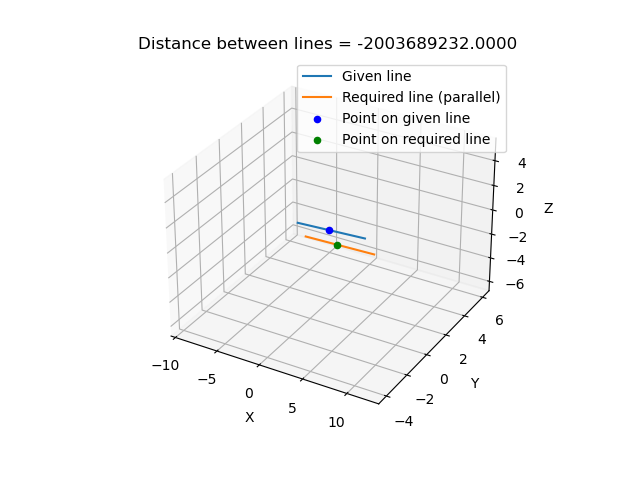
\includegraphics[width=0.85\textwidth,height=0.6\textheight,keepaspectratio]{Figs/Figure_7.png}
\end{frame}
\end{document}



